In this section, we describe our methodology, providing full details in later subsections. Ruxanne uses a pipeline for finding classes of pervasive patterns in Rust programs. This pipeline parses program versions, computes differences between them, embeds them in fixed-size datapoints, and then clusters these datapoints. After conducting a manual analysis on the obtained clusters, we refine them to obtain our proposed bug fix patterns.

We define a code change to be a modification to a program's source code that changes the program's abstract syntax tree (AST). A change pattern is a set of code changes that serves a specific purpose. Purposes include rectifying program behaviour with respect to a specific functional or non-functional requirement (bug-fixing patterns) as well as improving code readability or maintainability (refactoring patterns). In this work, we are interested in bug-fixing patterns. Thus, from now on, whenever we refer to code patterns, we mean bug-fixing patterns.

Our approach for automatically finding pervasive code patterns aims to find clusters of similar code patterns, using existing implementations of appropriate clustering algorithms. Work in this vein generally makes the assumption that clusters corresponds to classes of change patterns~\citep{hanam2016discovering,campos2019discovering,yang2022mining}. We thus want to associate code changes with datapoints; one of our contributions is a fixed-size embedding which highlights the important parts of a code change.


We implemented Ruxanne completely in Python. Our target repositories were the top 18 most-starred open source Rust projects on GitHub as of August 2021. We mined (using Pydriller) all the bug related commits and ran them through our pipeline; Section~\ref{sec:code_embedding} describes how we extracted fixed-size datapoints from the code changes, and Section~\ref{sec:mining} describes our mining methodology in depth. Then, we applied the DBSCAN clustering algorithm~\citep{ester1996density} on the resulting datapoints. Section~\ref{sec:clustering_data} describes clustering in detail, justifies our choice of DBSCAN for clustering, and explains how we tuned it to improve cluster quality. 

\subsection{\label{sec:code_embedding}Code Embedding}

To compute the contents of a change, we need two code revisions: the revision before the change, and the revision after it. After parsing these two revisions, we will have two ASTs. Tree diff algorithms can compute the differences between two arbitrary trees. When the trees are programs' abstract syntax trees, we call their diff an ASTDiff. An ASTDiff may include an arbitrary number of semantic changes, although a best practice is to include only one semantic change in a commit. Because that best practice is not universally followed, we are interested in finding the most important change within an ASTDiff, and embedding that change in our datapoints. Section~\ref{sec:parsing_programs} describes our program parsing process, and how we obtained ASTDiff from code changes. Sections~\ref{sec:path_extraction}~and~\ref{sec:weighting_scheme} provide a detailed explanation of how we select the most important semantic information out of an ASTDiff, which then allowed us to obtain clusters that contained similar datapoints. 

\subsubsection{\label{sec:parsing_programs}Parsing Programs}

Syn\footnote{\url{https://crates.io/crates/syn}} is a Rust crate built for the Rust procedural macro implementation. However, it includes a parser which is suitable for our purposes; we simply had to write a preprocessor to transform Syn AST output into Python dictionaries. Syn handles all of Rust. Each of our datapoints specifies whether any Syn non terminal (\texttt{NT}) is present or absent, i.e. containing one dimension per non terminal. However, we are also interested in change patterns that involve the borrow checker (BC), so we also add a dimension reflecting the presence of a set of BC-related elements (\texttt{BCE}) that we identified, e.g. \texttt{clone}, \texttt{Rc}, \texttt{Box}. The full list of \texttt{BCE} elements can be found in our replication package\footnote{\url{https://zenodo.org/record/7388618}}.

We parse two versions of a changed Rust file in a commit: the file before the commit and after it. This yields two Syn trees. Using the PLY tool\footnote{\url{https://www.dabeaz.com/ply/}} (a Python implementation of lex and yacc), we wrote a simple transformer from the serialized Rust AST to Python dictionaries. The change that transforms the first tree to the second one is the fix that was applied in the commit. To find this difference, we use dictdiffer\footnote{\url{https://dictdiffer.readthedocs.io/en/latest/}}, a Python library to find the diff of two Python dictionaries. Its output, in our context, is the ASTDiff.

\subsubsection{\label{sec:path_extraction}Path Extraction}



\begin{figure}[h]
\centering
\begin{tikzpicture}[scale=0.7, transform shape,every node/.style={draw},minimum height=0.7cm]

    
    %% Left AST
    
    \draw (-1.5,1.5) node[shape=rectangle, minimum width=3cm,minimum height=5.4cm, rounded corners=1ex, xshift=1.5cm, yshift=-2.5cm](context){};

    \node[draw, minimum height=0.5, fill=yellow!20] at (-0.74,1.7) {ASTDiff};
        
    \node[draw=none] at (0,1) {Context};
    
    \draw (0,0) node[](a1){ItemFn};
    \draw (0,-1) node[](a2){Local};
    \draw (0,-2) node[](a3){ExprCall};
    \draw (0,-3) node[](a4){args};
    
    
    \draw (-2,-5) node[shape=circle](null){null};
    
    
    \draw (0,-5) node[](b1){ExprReference};
    \draw (0,-6) node[](b2){Path};
    \draw (0,-7) node[](b3){Ident};
    \draw (0,-8) node[](b4){tail};
    
    \draw (3,-5) node[](c1){ExprMethodCall};
    \draw (3,-6) node[](c2){Path};
    \draw (3,-7) node[](c3){Ident};
    \draw (3,-8) node[](c4){head};
    
    
    \draw (5,-6.5) node[](d1){Ident};
    \draw (5,-7.5) node[](d2){clone};
    
    
    \draw[->]  (a1) -- (a2);
    \draw[->]  (a2) -- (a3);
    \draw[->]  (a3) -- (a4);
    
    \draw[->]  (context) -- (null);
    \draw[->]  (context) -- (b1);
    \draw[->]  (context) -- (c1);
    
    \draw[->]  (b1) -- (b2);
    \draw[->]  (b2) -- (b3);
    \draw[->]  (b3) -- (b4);
    
    \draw[->]  (c1) -- (c2);
    \draw[->]  (c2) -- (c3);
    \draw[->]  (c3) -- (c4);
    
    \draw[->]  (c1) -- (d1);
    \draw[->]  (d1) -- (d2);
    
    \draw [->, red] plot [smooth, tension=1] coordinates { (2,1) (2,-3) (1.4,-5) (1.4,-8.5)};
    
    \draw [->, green] plot [smooth, tension=1] coordinates { (2.5,1) (3,-3) (5,-5) (4,-6.5) (3.7,-8.5)};
    
    \draw [->, purple] plot [smooth, tension=1] coordinates { (3,1) (3.5,-3) (5.5,-5) (5.5,-8.5)};
    
    %% Arrow
    
    \node[draw=none] at (5.1,-2.7) {Path Extraction};
    \draw [-stealth,double,line width=2,color=blue!40](4.1,-3.2) -- (6.3,-3.2);
    
    %% Code at top right
    
    \node (codeA) [fill=yellow!20, rounded corners=1ex] at (10, 0) {%
    \centering
    \begin{minipage}{10cm}
    \centering
    \begin{lstlisting}[language=Rust, style=colouredRust]
      fn sample() {
        // ...
        -- let receiver = foo(arg1, tail, head)
        ++ let receiver = foo(arg1, &tail, head.clone())
        // ...
      }
    \end{lstlisting}
    \end{minipage}%
    };
    
    %% Paths at right
    
    \draw (7.5,-2.5) node[fill=red!30](e1){ItemFn};
    \draw (7.5,-3.5) node[fill=red!30](e2){Local};
    \draw (7.5,-4.5) node[fill=red!30](e3){ExprCall};
    \draw (7.5,-5.5) node[fill=red!30](e4){ExprReference};
    \draw (7.5,-6.5) node[fill=red!30](e5){Path};
    \draw (7.5,-7.5) node[fill=red!30](e6){Ident};
    
    \node[draw=none, color=red] at (7.5,-8.3) {Path 1};
    
    \draw (10.5,-2.5) node[fill=green!20](f1){ItemFn};
    \draw (10.5,-3.5) node[fill=green!20](f2){Local};
    \draw (10.5,-4.5) node[fill=green!20](f3){ExprCall};
    \draw (10.5,-5.5) node[fill=green!20](f4){ExprMethodCall};
    \draw (10.5,-6.5) node[fill=green!20](f5){Path};
    \draw (10.5,-7.5) node[fill=green!20](f6){Ident};
    
    \node[draw=none, color=green] at (10.5,-8.3) {Path 2};
    \node[draw=none, color=green] at (10.5,-8.3) {Path 2};
    
    \draw (13.5,-2.5) node[fill=purple!20](g1){ItemFn};
    \draw (13.5,-3.5) node[fill=purple!20](g2){Local};
    \draw (13.5,-4.5) node[fill=purple!20](g3){ExprCall};
    \draw (13.5,-5.5) node[fill=purple!20](g4){ExprMethodCall};
    \draw (13.5,-6.5) node[fill=purple!20](g5){Path};
    \draw (13.5,-7.5) node[fill=purple!20](g6){clone};
    \node[draw=none, color=purple] at (13.5,-8.3) {Path 3};
    
    \draw[->]  (e1) -- (e2);
    \draw[->]  (e2) -- (e3);
    \draw[->]  (e3) -- (e4);
    \draw[->]  (e4) -- (e5);
    \draw[->]  (e5) -- (e6);
    
    \draw[->]  (f1) -- (f2);
    \draw[->]  (f2) -- (f3);
    \draw[->]  (f3) -- (f4);
    \draw[->]  (f4) -- (f5);
    \draw[->]  (f5) -- (f6);
    
    \draw[->]  (g1) -- (g2);
    \draw[->]  (g2) -- (g3);
    \draw[->]  (g3) -- (g4);
    \draw[->]  (g4) -- (g5);
    \draw[->]  (g5) -- (g6);
    
    \end{tikzpicture}
    
    \caption{\label{fig:extraction}The ASTDiff (left) corresponds to the code change in the yellow box (top right). A DFS will identify three paths, shown in three different colors at right.}

\end{figure}
% yay tikz


The output of dictdiffer is a list of diffs, where each diff has three parts. The first part specifies the modification type:

\begin{itemize}
    \item `add': A new structure has been added to the tree; 
    \item `remove': A structure has been dropped from the tree; 
    \item `change': The content of a sub structure of the first tree has changed.
\end{itemize}

The second part identifies the context of the modification, that is, the path from the root of the tree to the subtree in which the modification has occured. The third part is the content of the change---terminals and nonterminals. Ruxanne looks for changes within each root-level scope (the Rust book\footnote{\url{https://doc.rust-lang.org/reference/items.html}} calls these root-level scopes the \textit{items} of a crate). That is, our assumption is that each change pattern occurs within one root-level scope. In this work, we chose to not handle patterns that involve changes in multiple functions or multiple files. However, our tool detects both continuous and non-continuous line changes within one scope.

Looking at the tree encoded in the content part of each diff, we realized that each path to a leaf represents one element contributing to the change. A Depth First Search allows us to collect all paths, and we return only the paths that we store in our datapoints (i.e. touching $\mathtt{NT} \cup \mathtt{BCE}$).

Figure~\ref{fig:extraction} illustrates path extraction on a simple change. The change replaces \verb+tail+ with \verb+&tail+ and \verb+head+ with \verb+head.clone()+. That is, after the change, the second argument passes a borrow of \verb+tail+ rather than sending the ownership of \verb+tail+ to the callee; and, the third argument sends a clone of head to the callee instead of sending head itself. A DFS on this tree yields three different paths, which we show in red, green, and purple. A path represents a sequence of involved non terminals. We found it crucial to record the order of nodes in the path, so that we could record that order in our datapoint embedding.

\paragraph{Code Embedding.} A key question is how to transform these paths to a fixed size datapoint. We need fixed-size datapoints, as they are a requirement for well-known centroid-based and density-based clustering algorithms~\citep{xu2005survey}. First, we need to define a fixed set of columns. The number of columns controls the amount of information we can embed in the datapoints. 

The most naive approach would be to only report the observed non terminals within the diff. That yields a fully order-insensitive representation. In such an embedding, for instance, there is no difference between two nested if statements and two if statements beside each other. On the other hand, theoretically, for full order-sensitiveness, we would need to embed all possible combinations of items from $\mathtt{NT} \cup \mathtt{BCE}$ as our dimensions, which yields a combinatorial explosion; this could potentially be reduced somewhat, but is still impractical. While we can implement a specific workaround to distinguish nested ifs (and we have done so), the general point about the large dimensionality of fully order-sensitive embedding still holds.

A reasonable work around would be to reduce $n$ from the full set of non terminals to a smaller set of categories (e.g. a category for larger entites like class or function definitions, and a category for smaller entities like statements and expressions), and then to record all possible combinations of these categories (similar to \cite{hanam2016discovering}). That approach reduces the number of dimensions and provides more reasonable and syntactically-correct combinations. However, it would still yield a sparse dataset. 

We propose a novel representation. Similar to the naive approach, we order-insensitively define the columns of our dataset as the set of items $\mathtt{NT} \cup \mathtt{BCE}$ we collected from Syn (the columns are constant across all Rust programs). However, to simulate order-sensitiveness, we add two more steps. First, we record the number of occurrences of items within the paths at each scope. The reason behind this decision is because a different order of program elements yields a different number of occurrences of underlying dimension. Second, we semi-automatically design a weighting scheme to prioritize non terminals that we think are more salient for Rust bugs. Section~\ref{sec:weighting_scheme}, immediately below, illustrates this approach on an example.

\subsubsection{\label{sec:weighting_scheme}Weighting Scheme}

\begin{figure}[h]
    \centering
    \begin{tikzpicture}[scale=0.7, transform shape, every node/.style={draw},minimum height=0.7cm]
        
        %% Left AST
        
        \draw (-1.5,1.5) node[shape=rectangle, minimum width=3cm,minimum height=5.4cm, rounded corners=1ex, xshift=1.5cm, yshift=-2.5cm](context){};
        
        \node[draw=none] at (0,1) {Context};
        
        \draw (0,0) node[](a1){ItemFn};
        \draw (0,-1) node[](a2){Local};
        \draw (0,-2) node[](a3){ExprCall};
        \draw (0,-3) node[](a4){args};
        
        
        \draw (-2,-5) node[shape=circle](null){null};
        
        
        \draw (0,-5) node[](b1){ExprReference};
        \draw (0,-6) node[](b2){Path};
        \draw (0,-7) node[](b3){Ident};
        \draw (0,-8) node[](b4){tail};
        
        \draw (3,-5) node[](c1){ExprMethodCall};
        \draw (3,-6) node[](c2){Path};
        \draw (3,-7) node[](c3){Ident};
        \draw (3,-8) node[](c4){head};
        
        
        \draw (5,-6.5) node[](d1){Ident};
        \draw (5,-7.5) node[](d2){clone};
        
        
        \draw[->]  (a1) -- (a2);
        \draw[->]  (a2) -- (a3);
        \draw[->]  (a3) -- (a4);
        
        \draw[->]  (context) -- (null);
        \draw[->]  (context) -- (b1);
        \draw[->]  (context) -- (c1);
        
        \draw[->]  (b1) -- (b2);
        \draw[->]  (b2) -- (b3);
        \draw[->]  (b3) -- (b4);
        
        \draw[->]  (c1) -- (c2);
        \draw[->]  (c2) -- (c3);
        \draw[->]  (c3) -- (c4);
        
        \draw[->]  (c1) -- (d1);
        \draw[->]  (d1) -- (d2);
        

        %% Tables
        
        \node[draw, minimum height=0.5, fill=yellow!20] at (-0.74,1.7) {ASTDiff};

        \node[draw, minimum height=0.5, fill=yellow!20] at (4.29,1.73) {Occurrences data};
        
        \matrix (table1) [table,text width=6em,nodes={scale=0.45,transform shape}] at (8.5,1)
        {
        Element & ItemFn  & Local & ExprCall & ExprReference & Path & Ident & ExprMethodCall & clone\\
        \# & 1 & 1 & 1 & 1 & 2 & 3 & 1 & 1 \\
        };
        
        \node[draw, minimum height=0.5, fill=yellow!20] at (4.12,-0.25) {Weighted data};
        
        \node[draw=none] at (8.2,0) {Multiply};
        \draw [-stealth,double,line width=1,color=blue!40](7,0.4) -- (7,-0.4);
        
        \matrix (table2) [table,text width=6em,nodes={scale=0.45,transform shape}] at (8.5,-1)
        {
        Element & ItemFn  & Local & ExprCall & ExprReference & Path & Ident & ExprMethodCall & clone\\
        weight & 0.0004 & 2.21e-05 & 8.68e-05 & 1 & 2.60e-05 & 2.76e-05 & 4.75e-05 & 1 \\
        };
        
        \node[draw=none] (circlepack) at (10.5,-6.2)
            {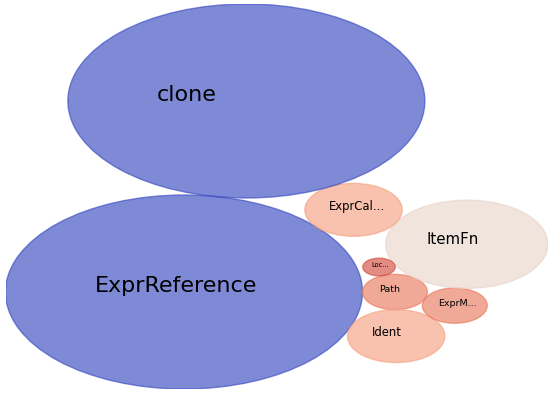
\includegraphics[width=0.7\textwidth]{circlepack.png}};
            
        
        \node[draw=none] at (9,-2.3) {Visualizing Essence};
        \draw [-stealth,double,line width=1,color=blue!40](7,-1.6) -- (7.5,-3.4);
        
        
        \end{tikzpicture}
        

    \caption{\label{fig:essence}Multiplying the number of occurrences of items observed in the tree by their respective weights results in the essence of change, visualized with a circle pack figure at bottom right. Vectors show (above) the number of occurrences and (below) weighted occurrence counts.}
\end{figure}

Our main requirement is that our datapoints summarize the key changes in ASTDiffs---a datapoint should foreground the most important change in a diff. For instance, the purple (right-most) path in Figure~\ref{fig:extraction} could be described as a change in a local variable declaration; a change in a function call; calling a method of one of the function arguments; or calling clone() on one of the function arguments. The last description, in our opinion, is the most useful one, and we designed our weighting scheme to embed this value judgment.
We made two observations about changes. First, we saw that items (non terminals or BC-related elements) that occurs closer to AST leaves tend to be more semantically important. Second, and relatedly, items closer to the root tend to be repeated in all the paths within one ASTDiff (e.g. ItemFn, Local, ExprCall in Figure~\ref{fig:extraction}). We thus want to prioritize items that tend to occur closer to leaves and de-prioritize items that tend to occur closer to roots.

To design our weighting scheme, we collected empirical data about locations of item occurrences in a corpus. Specifically, we mined 20 of the most recent bug related commits of the same projects described in Table~\ref{table:repos}, and ran them through our pipeline. We recorded the total number of occurrences of each item. Then, if $\# i$ is the number of occurences of $i$, we gave $i$ a weight of $1/\# i$. Because items that occur closer to the root also occur more often, per our observation, this gives higher weights to items that occur infrequently, i.e. closer to the leaves. Items that occur often and have lower weights are, we believe, less important in describing a change.

Furthermore, as we wanted to make sure that our tool captures patterns related to the Rust borrow checker, we manually increased the weights of the \texttt{BCE} items. The manual adjustment is why we characterize our weighting scheme as semi-automatically designed. The final weights can also be found in our replication package.

Multiplying the number of occurrences of all observed items in a change by their respective weights results in a vector of numbers. We call this vector the \emph{essence of change}. In this vector, the value for each item shows its importance in the change. Figure~\ref{fig:essence} shows the process of computing the essence of the code change that we saw in Figure~\ref{fig:extraction}. We have visualized this essence vector using a circle pack figure. The radius of each circle corresponds to the importance of the item inside it.

\subsection{\label{sec:mining_repositories}Mining Repositories}
\label{sec:mining}

\begin{table}
\caption{\label{table:repos} We chose the 18 most-starred Rust projects on GitHub as target repositories for mining.
}
\begin{tabular}{l r r r r}
    Project Name & Stars(k) & LOC & \# Commits & Avg. Code Churn \\
    denoland/deno & 85.9 & 146055 & 8026 & 49.22 \\
    tauri-apps/tauri & 52.5 & 50014 & 3041 & 31.67 \\
    alacritty/alacritty & 42.4 & 30124 & 2036 & 27.53 \\
    sharkdp/bat & 37.6 & 9496 & 2457 & 59.13 \\
    starship/starship & 29.3 & 34888 & 2379 & 25.1 \\
    rust-lang/rustlings & 30.6 & 5067 & 1466 & 8.92 \\
    meilisearch/meilisearch & 30.2 & 25981 & 4029 & 279.7 \\
    sharkdp/fd & 24.9 & 6542 & 1068 & 12.2 \\
    swc-project/swc & 24.2 & 346501 & 5884 & 44.34 \\
    yewstack/yew & 24.5 & 44295 & 2280 & 21.79 \\
    xi-editor/xi-editor & 19.6 & 39292 & 2105 & 28.67 \\
    AppFlowy-IO/AppFlowy & 28.4 & 57646 & 3321 & 29.49 \\
    firecracker-microvm/firecracker & 19.6 & 82021 & 3620 & 58.26 \\
    nushell/nushell & 21.1 & 163562 & 6088 & 22.38 \\
    ogham/exa & 19.5 & 10852 & 1558 & 11.99 \\
    SergioBenitez/Rocket & 18.7 & 68952 & 2135 & 19.75 \\
    rustdesk/rustdesk & 30.2 & 48115 & 2620 & 72.81 \\
    tokio-rs/tokio & 17.9 & 121400 & 3101 & 28.87 
\end{tabular}
\end{table}
   

Now that we have set up our code analysis pipeline, we can start mining the Rust repositories. We target the top 18 most-starred Rust projects on GitHub, at the time of data collection. Table~\ref{table:repos} summarizes our benchmarks. Because we are interested in changes, we computed (using process metrics provided by our mining library) the average code churn of the files within the projects. denoland/deno and swc-project/swc are the projects with largest number of LOCs and highest average code churn, respectively. Unsurprisingly, we captured a lot of instances from these two projects in our final clusters.

We used the Pydriller~\citep{spadini2018pydriller} library to mine software repositories. Pydriller provides APIs to extract commits from a Git repository and to search through different revisions of files. Algorithm~\ref{alg} shows how we used Pydriller to run the target repositories through our code analysis pipeline and populate two databases: one for borrow-checker related patterns (which involve items in \texttt{BCE}) and one for general patterns (which don't). For each repository, we search all commits that include bug-fixing related keywords within their commit messages. Here, we chose bug-fixing related keywords based on the set introduced in \cite{zhang2018empirical}, excluding `nan' and `inf'. 


Next, we collect a pair of revisions for each Rust file. The pair includes the state of the file before the commit and after the commit ($f_a, f_b$). After parsing each revision and computing the ASTDiff, we can compute the fixed sized datapoint $\mathit{DP}$. If the datapoint contains borrow-checker related keywords, we put it in the BC-related database $D_b$; otherwise, we put it in the general code changes database $D_g$. In both cases, we augment the datapoint with the commit hash, filename, and the scope in which the change happened. For BC-related code changes, we also store the detected BC-related keywords. In summary, a datapoint is a tuple containing essence values for each element in $\mathtt{NT} \cup \mathtt{BCE}$ plus metadata about the change (e.g. commit hash, filename, etc.). Now our databases are ready for clustering and categorization.

\begin{algorithm}
\caption{\label{alg} Mining Algorithm}
\hspace*{2mm} \textbf{Input:} $R$ (target repositories)  \\
\hspace*{2mm} \textbf{Output:} $D_g$ (General code changes) \\
\hspace*{2mm} \textbf{Output:} $D_b$ (BC-related code changes)
\begin{algorithmic}
\State $D_g \leftarrow \phi$
\State $D_b \leftarrow \phi$
\For{$r \in R$}
    \For{$c \in \textsc{ExtractCommits}(r)$}
        \If{$c.msg$ contains bug fixing related keywords}
            \For{$\{f_b, f_a\} \in \textsc{GetModifiedRustFiles}(c)$}
                \For{$e \in \textsc{ASTDiff}(\textsc{Parse}(f_b), \textsc{Parse}(f_a))$}
                    \State $\textit{DP} \leftarrow \textsc{GetDataPoint}(e)$
                    \State $\textit{DP} \leftarrow c.\textit{hash} \cup f_a.\textit{name} \cup e.\textit{scope} \cup \textit{DP} $
                    \If{$\textsc{IsBCRelated}(e)$}
                        \State $\textit{DP} \leftarrow \textsc{GetBCKeyword}(e) \cup \textit{DP} $
                        \State $D_b \leftarrow D_b \cup \textit{DP}$
                    \Else
                        \State $D_g \leftarrow D_g \cup \textit{DP}$
                    \EndIf
                \EndFor
            \EndFor
        \EndIf
    \EndFor
\EndFor
\end{algorithmic}
\end{algorithm}

\subsection{\label{sec:clustering_data}Clustering Data}
\label{sec:clustering}

Having collected our datapoints, our next task is to cluster them so that we can categorize bug patterns. Like \cite{hanam2016discovering}, we use the DBSCAN clustering algorithm for two main reasons. Firstly, in contrast to k-means, it does not require the number of clusters in advance as an input to the algorithm. Secondly, it is a density-based clustering method, which means that it detects arbitrarily shaped clusters; centroid-based methods like k-means can't detect such clusters.

DBSCAN takes two tuneable parameters. The first parameter $\epsilon$ indicates a radius distinguishing core points, border points, and outliers. The second parameter $Z$ is the minimum number of points per cluster. We ran DBSCAN using different combinations of these two parameters. In Figure~\ref{fig:clustering}, we show nine different experiments, with their respective parameter values. Each subplot specifies, for both $D_g$ and $D_b$, the number of clustered points, noise points, and the number of clusters.

\begin{figure}[h]
\centering
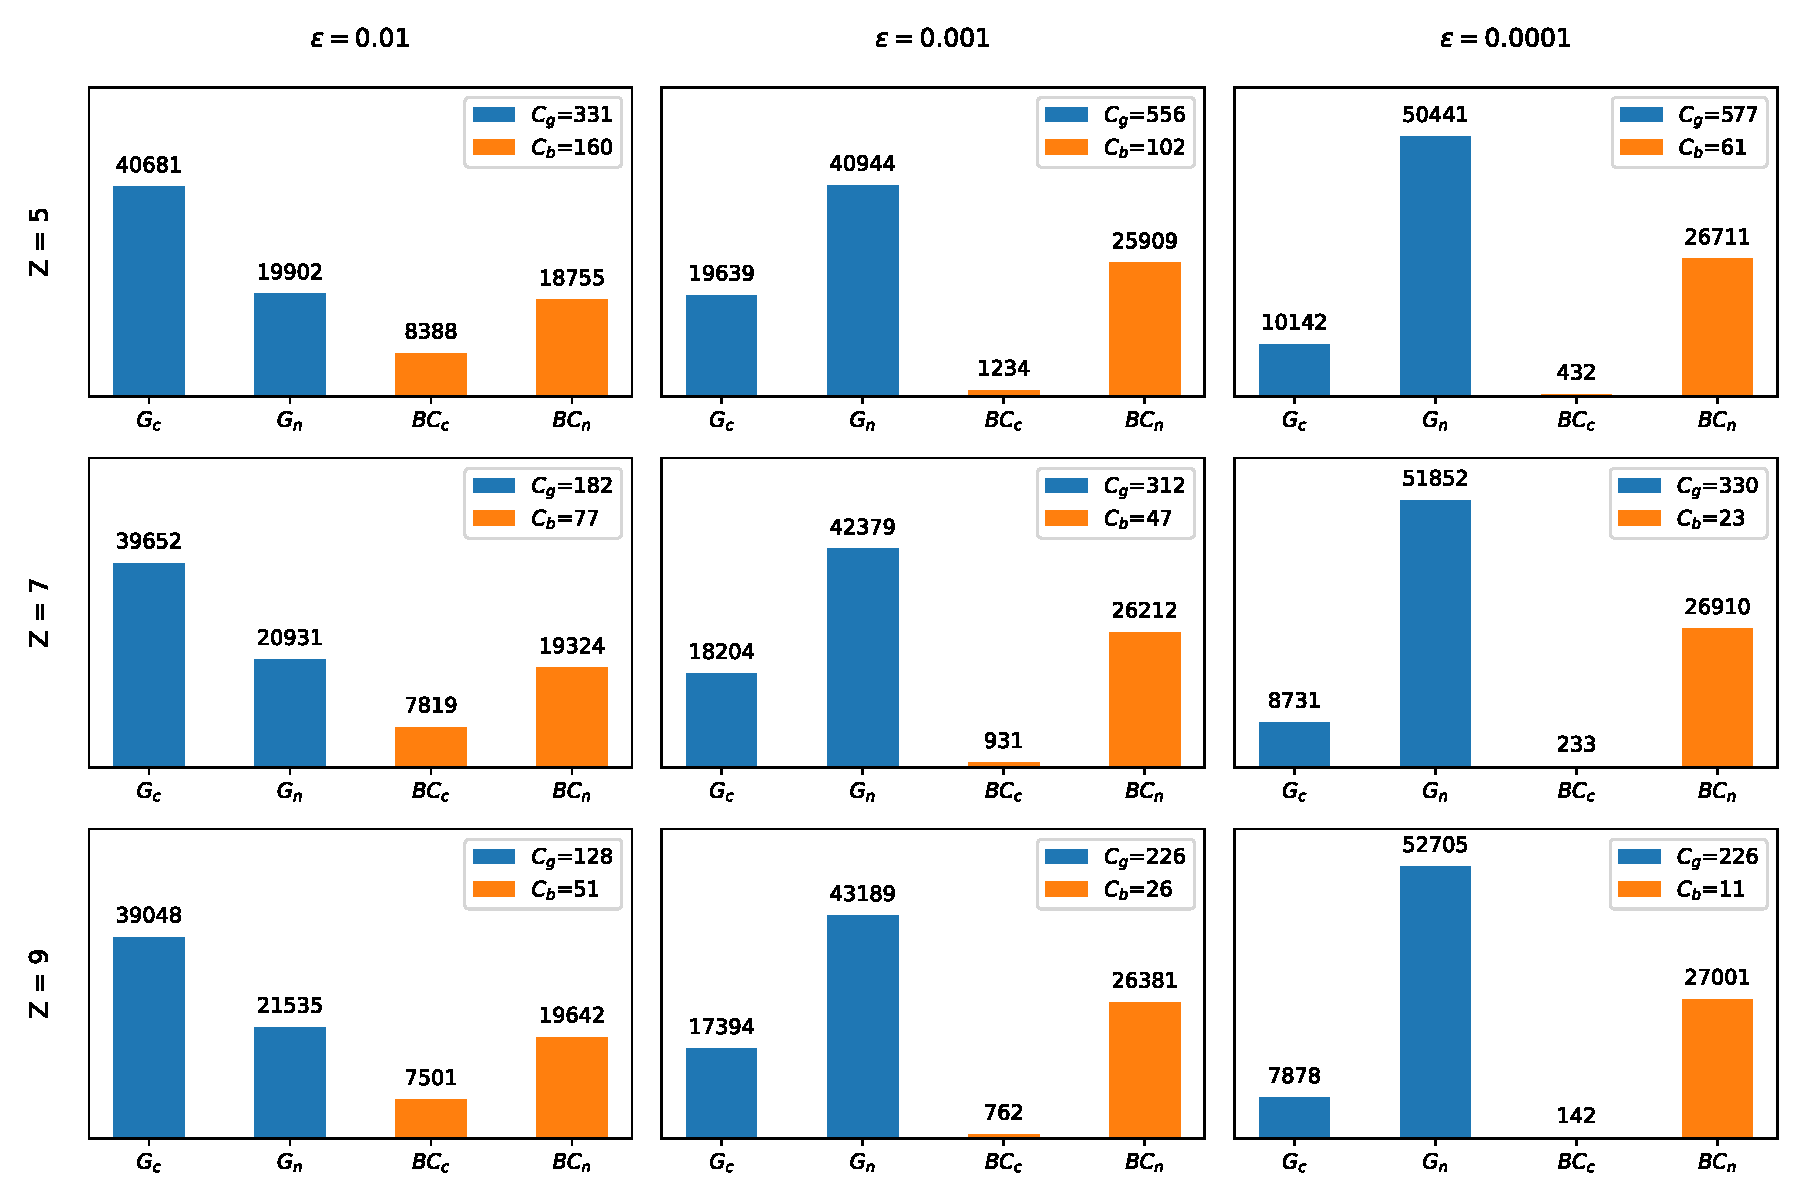
\includegraphics[width=1\textwidth]{clusters.pdf}
\caption{\label{fig:clustering} Clustering results with nine different combinations of parameters $\epsilon$ and $Z$, respectively separated in columns and rows. In each subplot, the two blue bars in the left respectively indicate the number of clustered ($G_c$) and noise ($G_n)$ datapoints (the number is shown above each bar) after applying clustering on general database $D_g$. The two orange bars in the right show similar data but for the borrow-checker database $D_{b}$. In each subplot's legend, $C_g$ and $C_b$ show the number of clusters obtained from $D_g$ and $D_b$, respectively}
\end{figure}

As a general rule, lower $Z$ would allow more groups of nearby points to be considered to be clusters, resulting in a higher number of clusters. A large $\epsilon$ would widen the search radius, allowing more points to fall in the clusters, which results in a reduction of the number of noise points. However, such a choice might put points from different patterns inside the same cluster, resulting in ineffective clustering. Alternatively, a small $\epsilon$ would tighten the ring of search, possibly separating clusters which essentially manifest the same code changes. Also, if $\epsilon$ is really small, the clustering algorithm might not detect some clusters at all, resulting in a reduction of the number of clusters. 

\subsubsection{\label{sec:manual_analysis_parameter_tuning}Manual Analysis for parameter tuning}

Since both large and small values of $\epsilon$ would steer us away from obtaining meaningful clusters, we felt the need to carry out a manual analysis of clusters for better parameter tuning. In the manual analysis, we randomly picked 50 clusters; from each cluster we randomly chose 10 datapoints. The person analyzing the cluster (the first author) then looked at the code and specified the clusters that contained more than five datapoints showing similar patterns. After conducting the manual analysis, we decided to use $\epsilon=0.0001, Z=5$ and $\epsilon=0.001, Z=5$, as our clustering parameters for $D_g$ and $D_b$, resulting in 577 and 102 clusters, respectively. As a final step, we excluded clusters that contained datapoints from fewer than 3 projects. That is because we wanted our clusters to contain cross-project (e.g. potentially generalizable) patterns as much as possible.  

\subsubsection{\label{sec:manual_analysis_cluster_selection}Manual Analysis for cluster selection}
% 3 types, refactoring dropped

Like \cite{yang2022mining}, and following the definitions of \cite{cotroneo2019analyzing}, we divide the clusters in three different groups:

\begin{itemize}
    \item bug-fix: ``The changed code actually fixes the behavior of software, which can represent fixes for a bug type''. We include here changes that improve program performance, as they fix the behaviour of the software.

    \item fix-induced: ``The changed code is a group of bug-fixing code changes but not representing an actual bug fix, e.g., adding new input parameters to a method, the method signature and method call must be changed correspondingly''.
    
    \item refactoring: ``the changed code does not modify the software behavior, e.g., for better readability or encapsulation''.
\end{itemize}

In this work, we were only interested in the first two groups and ignored clusters for refactoring changes. Also, we prefer reporting clusters that manifest more-specific patterns. An abstract pattern as opposed to a more-specific pattern can account for many changes in the programs. We use our judgment to prioritize patterns that we deem more specific. For instance, we deem the pattern `Changing a clone of a variable to a borrowing of it in a function argument' more specific than `Changing a statement in a function's body':

\begin{lstlisting}[language=Rust, style=colouredRust]
// First Pattern
-- foo1(arg.clone);
++ foo1(&arg);

// Second Pattern
fn foo2() {
--  stmt1;
++  stmt2;
}

\end{lstlisting}


In our manual analysis, we randomly picked 50 datapoints of each cluster. If the cluster had fewer than 50 datapoints, we analyzed all of the datapoints in the cluster. Regarding general patterns, we obtained 577 clusters, out of which 428 included cross-project patterns. Of these 428 clusters, 35 clusters included more than 50 points. That is, we did not do random sampling for 393 clusters, we just manually analyzed all the datapoints in them. Regarding BC-related patterns, out of 102 obtained clusters, 49 clusters included cross-project patterns. Only 4 of these 49 clusters included more than 50 datapoints, therefore, we only did a random sampling for 4 clusters. For each cluster, we read the code and the bug reports of the datapoints (if they existed). If we judged that the members of a cluster fit into a pattern, we wrote a natural language description of that cluster. Considering the descriptions, we linked similar clusters together as possible candidates for merging. We considered these candidates and carried out appropriate ones. Finally, we selected 20 of the remaining clusters---the ones that manifested more-specific changes. Sections~\ref{sec:common_patterns}~and~\ref{sec:bc_patterns} present our clusters.
